\subsection{Higher research productivity}
\label{subsec:rewrite-rsi-half-decline}

I now compare the transitional dynamics for the four elasticities of substitution under a relative high parameter of research productivity ($\chi=7.5$). This parameter is only relevant for the short-behavior, as the long-run growth rates and do not depend on this parameter. All four economies inherit the pre-RSI balanced growth paths described in Section~\ref{subsec:rewrite-rsi-activation}. Table~\ref{tab:rewrite-rsi-parameters} reports their common parameters and elasticity-specific initial capital stocks. The objective is to show how the four scenarios differ from one another along the transition. The long-run behavior has already been characterized in Section \ref{sec:rewrite-regimes}. 


% Generated by scripts/report_rewrite_illustrative_rsi.py; do not edit numbers.
Immediately after activation, output-per-person growth is $1.61\%$, $2.68\%$, $2.98\%$, $4.47\%$ for $\sigma=0.90,1,1.10,1.50$, respectively, compared with $1\%$ before activation.
These are changes in growth rates, not jumps in output levels.

At $\sigma=1.50$, initial research expenditure is $3.05\%$ of output and developer net profit is $0.24\%$ of output. Labor's income share reaches half its initial value after about 47 years. At year 500, output-per-person growth is $3.24\%$, wage growth is $2.50\%$, and the interest rate is $7.24\%$.

The corresponding long-run limits are $3.13\%$, $2.42\%$, and $7.13\%$, respectively; these limits are the same in both exercises.

At unit elasticity, first-year research expenditure is $0.182\%$ of output and the AI-service price falls by $39.6\%$ over the first 27 months. Both are outcomes of the exercise, not calibration targets.


Higher research productivity produces a sizable initial increase in growth in all four economies. This increase eventually vanishes in the three
labor-bottleneck cases. In the AI-dominated case, growth instead rises further before declining toward its higher long-run rate. The simulation thus distinguishes an initial response to RSI from the subsequent divergence between growth regimes.

Figures~\ref{fig:rewrite-rsi-half-accumulation}--\ref{fig:rewrite-rsi-half-distribution}
show the first ten years and years 10--500 separately. Dotted horizontal
lines mark the analytical limits for $\sigma=1.50$.
Section~\ref{subsec:rewrite-rsi-research-share} uses the same presentation
with lower research productivity. Vertical scales may differ between
the two exercises to keep their transitions legible.

\begin{figure}[H]
 \centering
 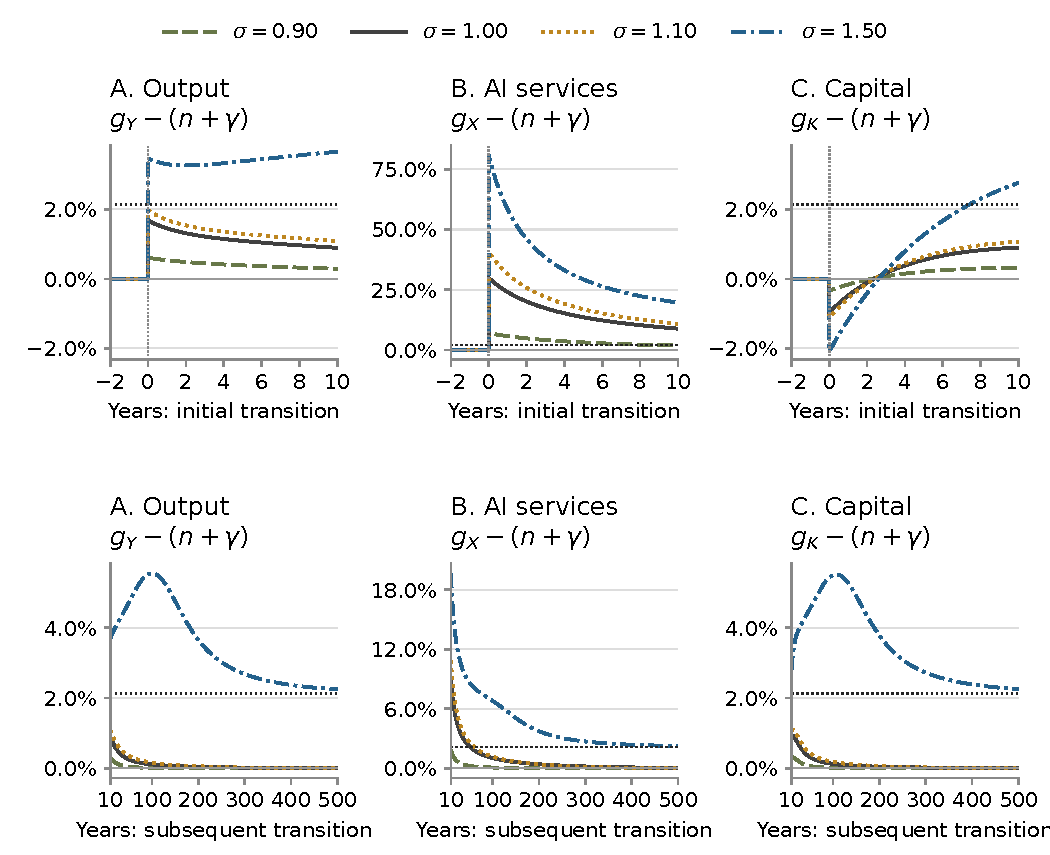
\includegraphics[width=\textwidth]{figures_rewrite/equilibrium_rsi_chi_7_5_accumulation_growth_windows.pdf}
 \caption{Higher research productivity ($\chi=7.5$): growth of output,
 AI production services, and capital per unit of effective labor. Rates
 are instantaneous annual rates. The upper row shows two pre-event years
 and years 0--10; the lower row shows years 10--500. Panels A and C share
 a scale within each row. The vertical line marks RSI activation.}
 \label{fig:rewrite-rsi-half-accumulation}
\end{figure}

\begin{figure}[H]
 \centering
 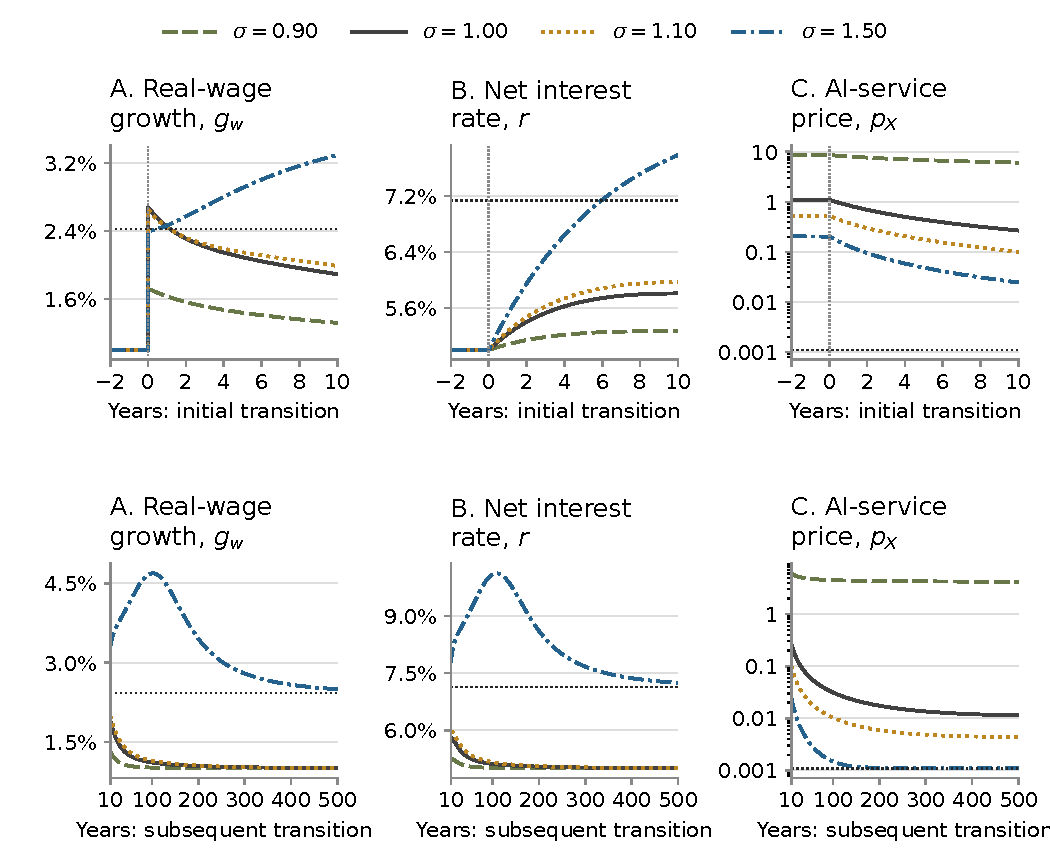
\includegraphics[width=\textwidth]{figures_rewrite/equilibrium_rsi_chi_7_5_growth_returns_windows.pdf}
 \caption{Higher research productivity ($\chi=7.5$): real-wage growth,
 the net interest rate, and the AI-service price. Rates are annual;
 the price is in final-good units on a logarithmic scale.
 The vertical line marks RSI activation.}
 \label{fig:rewrite-rsi-half-prices}
\end{figure}

\begin{figure}[H]
 \centering
 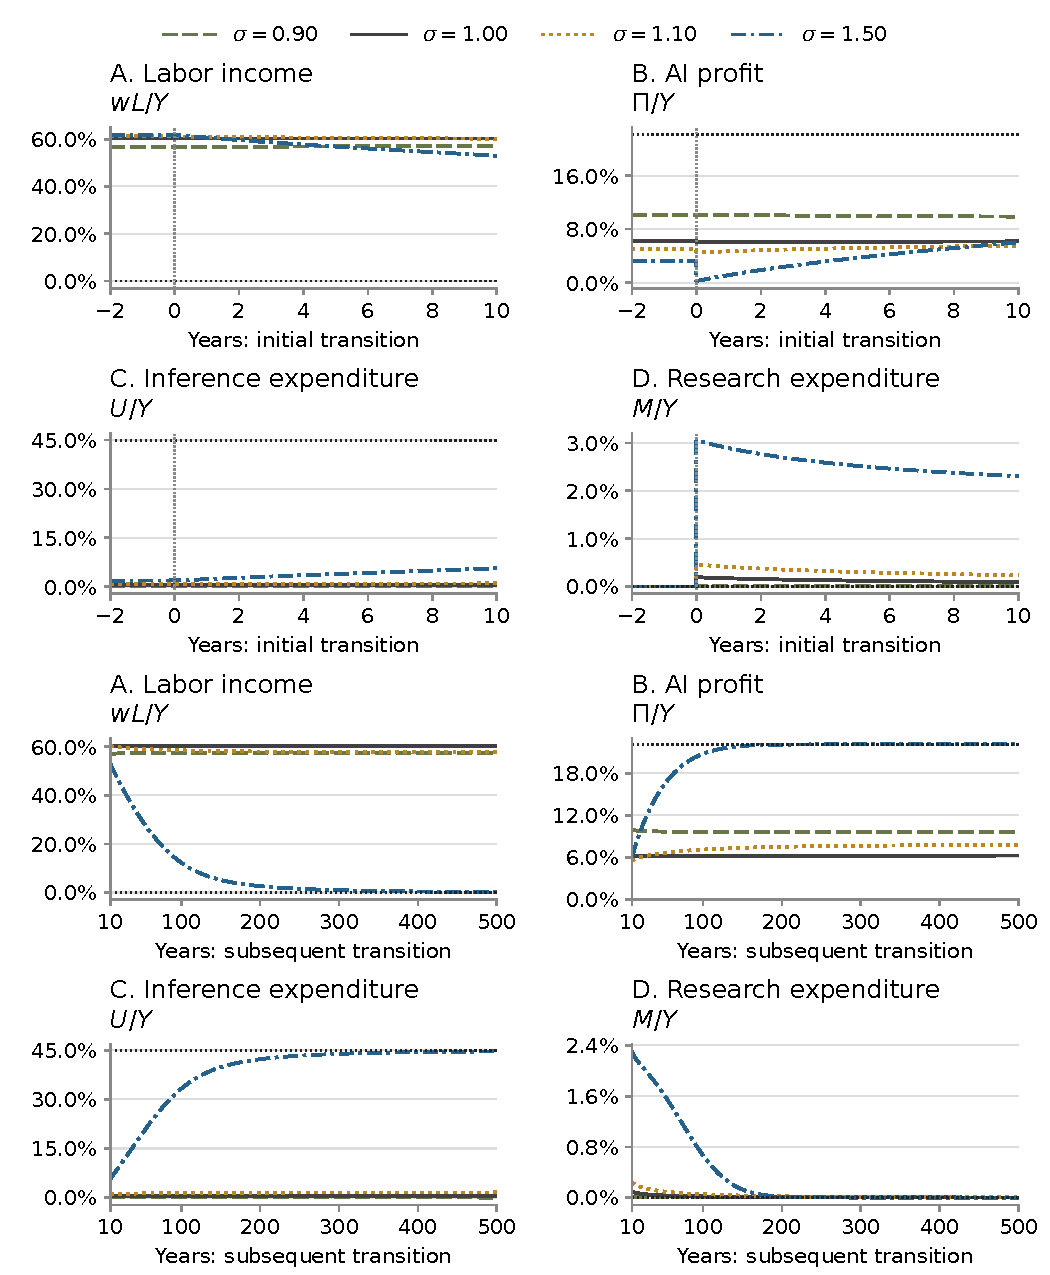
\includegraphics[width=\textwidth]{figures_rewrite/equilibrium_rsi_chi_7_5_ai_distribution_windows.pdf}
 \caption{Higher research productivity ($\chi=7.5$): labor income,
 AI net profit, inference expenditure, and research expenditure relative
 to output. The first two rows show the pre-event BGP and years 0--10;
 the last two show years 10--500. The omitted gross capital share
 remains $\alpha=0.33$.}
 \label{fig:rewrite-rsi-half-distribution}
\end{figure}
